\documentclass{article}

\usepackage{fullpage}
\usepackage{graphicx}
\usepackage{hyperref}
\usepackage{xepersian}

\newcommand{\assignment}{پروپوزال پروژه: پیش‌بینی قیمت خانه‌های شهر تهران}
\newcommand{\course}{مبانی سیستم‌های هوشمند}
\newcommand{\faculty}{دانشکده مهندسی برق}
\newcommand{\university}{دانشگاه صنعتی خواجه نصیرالدین طوسی}

\hypersetup{colorlinks=true, linkcolor=blue, urlcolor=magenta}

\settextfont[Path={fonts/}, BoldFont={IRLotusICEE_Bold.ttf}, BoldItalicFont={IRLotusICEE_BoldIranic.ttf}, ItalicFont={IRLotusICEE_Iranic.ttf}, Scale=1.2]{IRLotusICEE.ttf}
\setlatintextfont[Path=fonts/, BoldFont={LiberationSerif-Bold.ttf}, BoldItalicFont={LiberationSerif-BoldItalic.ttf}, ItalicFont={LiberationSerif-Italic.ttf}, Scale=1]{LiberationSerif-Regular.ttf}

\title{\assignment}
\author{
    محمدامین توفیق \\
    \texttt{m.toufigh@email.kntu.ac.ir} \\
    \and
    محمدمهدی کرمی \\
    \texttt{mmehdi.karami@email.kntu.ac.ir}
}
\date{\university \\
\faculty \\
\course}

\begin{document}

\maketitle

% Introduction Section
\section{مقدمه}
در این پروژه، قصد داریم با استفاده از روش‌های یادگیری ماشین و داده‌کاوی، مدل‌هایی برای پیش‌بینی قیمت خانه‌ها در تهران توسعه دهیم. این مدل‌ها با استفاده از داده‌های جمع‌آوری‌شده از یک یا چند سایت معتبر که آگهی‌های فروش خانه در تهران را منتشر می‌کنند، تحلیل شده و ویژگی‌های کلیدی مؤثر بر قیمت استخراج خواهند شد.

% Objectives Section
\section{اهداف پروژه}
هدف اصلی این پروژه، پیش‌بینی قیمت خانه‌های شهر تهران با استفاده از مدل‌های هوش مصنوعی و به ویژه شبکه‌های عصبی است. برای دستیابی به این هدف، مراحل مختلفی انجام خواهند شد که شامل جمع‌آوری داده، تحلیل و استخراج ویژگی‌ها، آموزش مدل‌ها و ارزیابی آن‌ها به شرح زیر است:

\begin{enumerate}
    \item جمع‌آوری داده‌ها از وب‌سایت‌های معتبر تهران با استفاده از تکنیک‌های استخراج داده از وب
    \item تحلیل داده‌ها و استخراج ویژگی‌های موثر بر قیمت خانه‌ها
    \item آموزش مدل‌های یادگیری ماشین برای پیش‌بینی قیمت خانه
    \item ارزیابی عملکرد مدل‌ها و بهبود آن‌ها با استفاده از تکنیک‌های مختلف مانند تنظیم پارامترها، استفاده از الگوریتم‌های بهینه‌سازی و ارزیابی مدل‌های مختلف
    \item طراحی و پیاده‌سازی یک رابط کاربری گرافیکی برای استفاده از مدل پیش‌بینی
    \item تست مدل در سناریوهای مختلف و ارائه پیشنهادات بهینه‌سازی بر اساس نتایج به‌دست‌آمده
\end{enumerate}

% Methodology Section
\section{روش‌های تحقیق}
در این پروژه، ابتدا داده‌ها از منابع معتبر جمع‌آوری خواهند شد، سپس به آنالیز داده‌ها و مدل‌سازی پرداخته می‌شود. مراحل تحقیق به شرح زیر است:

\subsection{جمع‌آوری داده‌ها}
داده‌ها از منابع معتبر بازار مسکن تهران مانند \href{https://kilid.com/}{کیلید} جمع‌آوری خواهند شد. ویژگی‌های داده‌ها شامل مساحت خانه، تعداد اتاق‌ها، سال ساخت، موقعیت جغرافیایی، و قیمت نهایی می‌باشد. برای جمع‌آوری این داده‌ها از تکنیک‌های \lr{Web Scraping} استفاده خواهیم کرد، که با استفاده از کتابخانه‌های پایتون مانند \lr{BeautifulSoup} و دیگر ابزارها، داده‌های مورد نظر را از صفحات وب استخراج می‌کنیم.

\begin{figure}
    \centering
    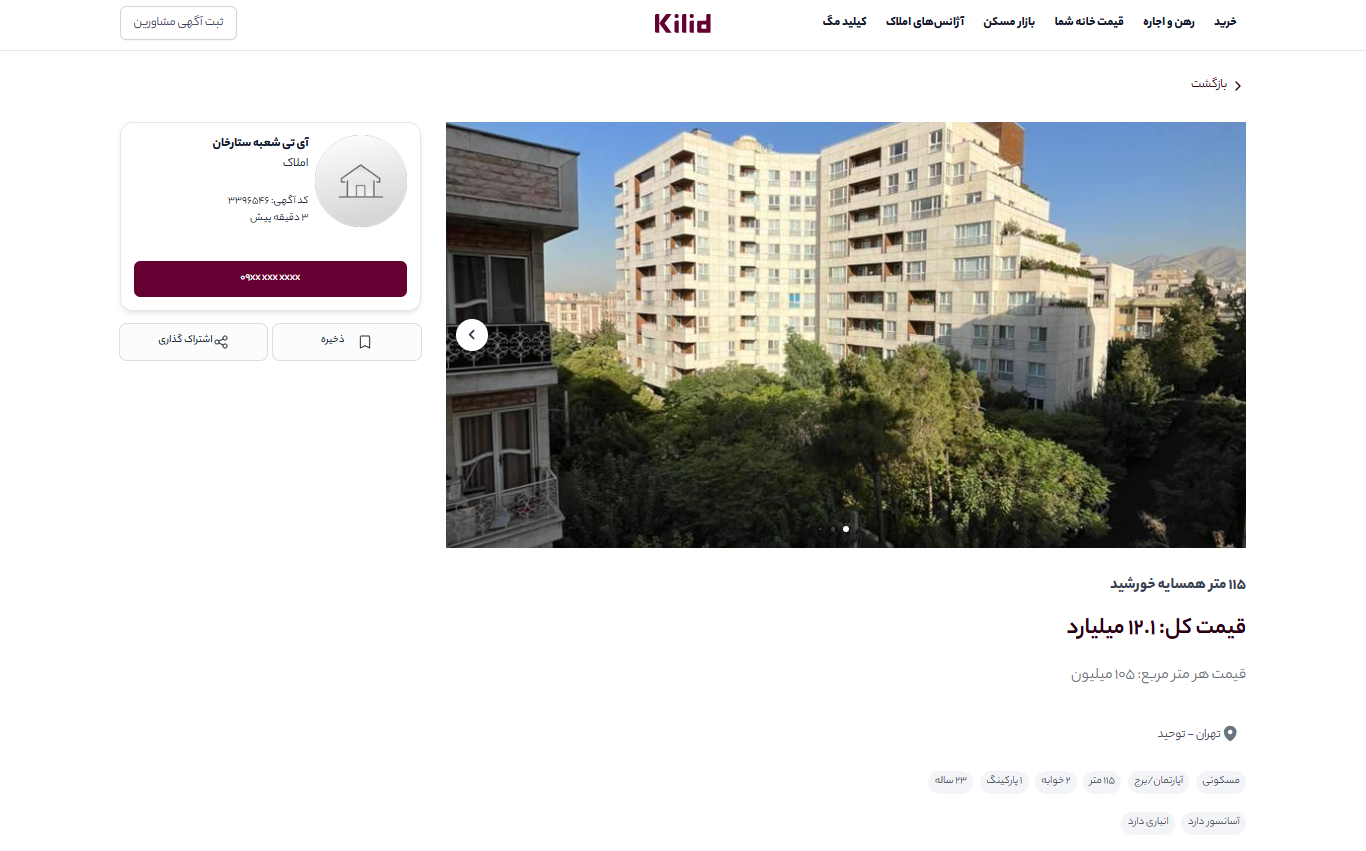
\includegraphics[width=0.7\textwidth]{img/sample-ad.png}
    \caption{نمونه‌ای از آگهی فروش خانه در سایت \href{https://kilid.com/}{کیلید}}
    \label{fig:sample-ad}
\end{figure}

\subsection{تحلیل داده‌ها}
داده‌ها بررسی می‌شوند. داده‌های \lr{null} یا داده‌هایی که مشکل دارند تحلیل و بر اساس بهترین تصمیم حذف یا ویرایش می‌شوند. همچنین، داده‌های پرت بررسی شده و در صورت نیاز حذف خواهند شد. تحلیل همبستگی برای شناسایی ویژگی‌های کلیدی انجام می‌شود و ویژگی‌های موثر بر قیمت خانه‌ها انتخاب خواهند شد.

\subsection{مدل‌سازی}
شبکه‌های عصبی به عنوان مدل اصلی استفاده خواهند شد. این مدل برای پیش‌بینی قیمت خانه‌ها با استفاده از ویژگی‌های استخراج‌شده آموزش خواهد دید. ارزیابی مدل‌ها با استفاده از معیارهای مناسب انجام می‌شود. همچنین، روش‌های مختلف مدل‌سازی بررسی می‌شوند و در صورت نیاز ترکیب می‌شوند تا بهترین نتیجه حاصل گردد.

\subsection{رابط کاربری}
رابط گرافیکی ساده‌ای طراحی خواهد شد که کاربران بتوانند ویژگی‌های خانه را وارد کرده و قیمت پیش‌بینی‌شده را مشاهده کنند. این رابط کاربری به صورت یک اپلیکیشن وب یا دسکتاپ خواهد بود که از طریق آن کاربران می‌توانند به راحتی از مدل پیش‌بینی استفاده کنند.

% Conclusion Section
\section{نتیجه‌گیری}
پیش‌بینی قیمت خانه‌ها در تهران با استفاده از یادگیری ماشین و تحلیل داده‌ها، مدل دقیقی برای پیش‌بینی قیمت خانه‌ها ارائه خواهد کرد. علاوه بر این، رابط کاربری طراحی‌شده به کاربران این امکان را می‌دهد که به سادگی از مدل پیش‌بینی قیمت خانه استفاده کنند و تصمیمات بهتری اتخاذ نمایند.

\end{document}
